\subsection{Результаты}
В результате обучения, были получены оптоэлектронные сети для трёх вариаций пространственной когерентности: $50$ мкм, $1000$ мкм, $3000$ мкм. Значение $50$ мкм было выбран потому, что солнечный свет обладает именно такой пространственной когерентностью. Основные результаты представлены на рисунке \ref{ris:Results}.
\begin{figure}[h]
	\centering{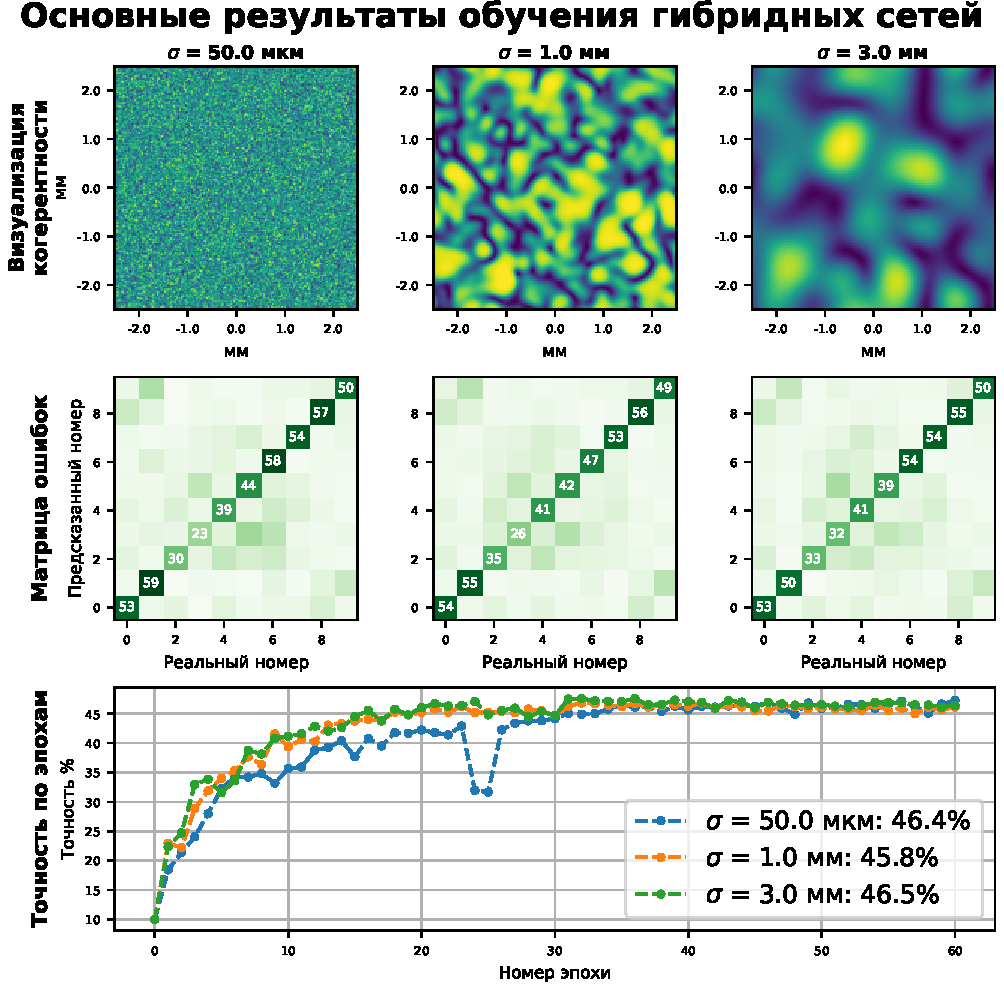
\includegraphics[width=1.0\linewidth]{figures/ModelResults.pdf}}
	\caption{Результаты обучения гибридных нейронных сетей. Первый ряд -- визуализации конкретной реализации фазы некогерентного поля. Второй ряд -- матрица ошибок: цвет отображает процент ответов, числа на диагонали отображают процент правильных ответов. Третий ряд -- график зависимости точности от номера эпохи для трёх моделей.}
	\label{ris:Results}
\end{figure}
По этим результатам видно, что в не зависимости от степени пространственной когерентности, модели показали одинаковый результат при большом количестве эпох обучения. Маленькая точность для классов $2$, $3$, $4$, $5$ связана со схожестью изображений этих классов.
На рисунках \ref{ris:ModelPhase}, \ref{ris:ModelAmplitude} изображены характеристики модуляции фазы и амплитуды моделей.
\begin{figure}[h]
	\centering{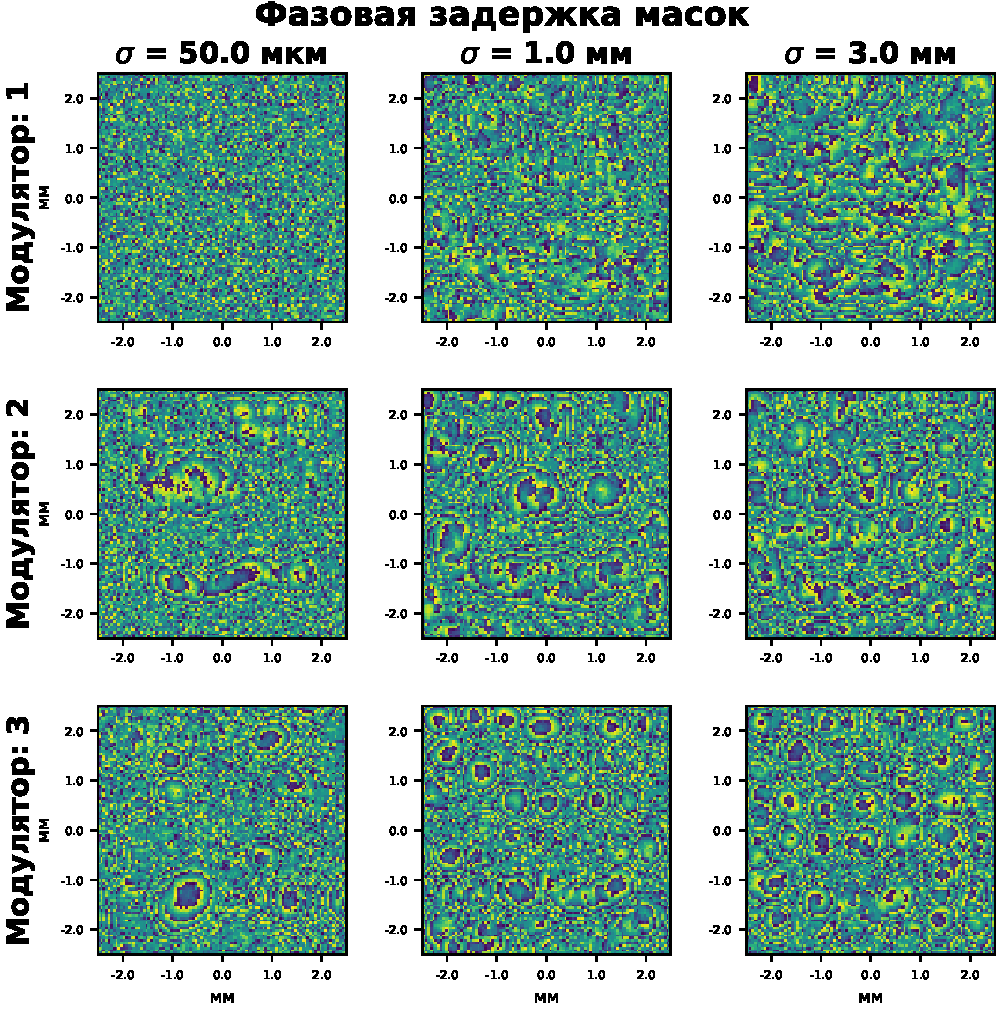
\includegraphics[width=1.0\linewidth]{figures/ModelPhase.pdf}}
	\caption{Дополнительная задержка фазы на неоднородностях масок моделей.}
	\label{ris:ModelPhase}
\end{figure}
\begin{figure}[h]
	\centering{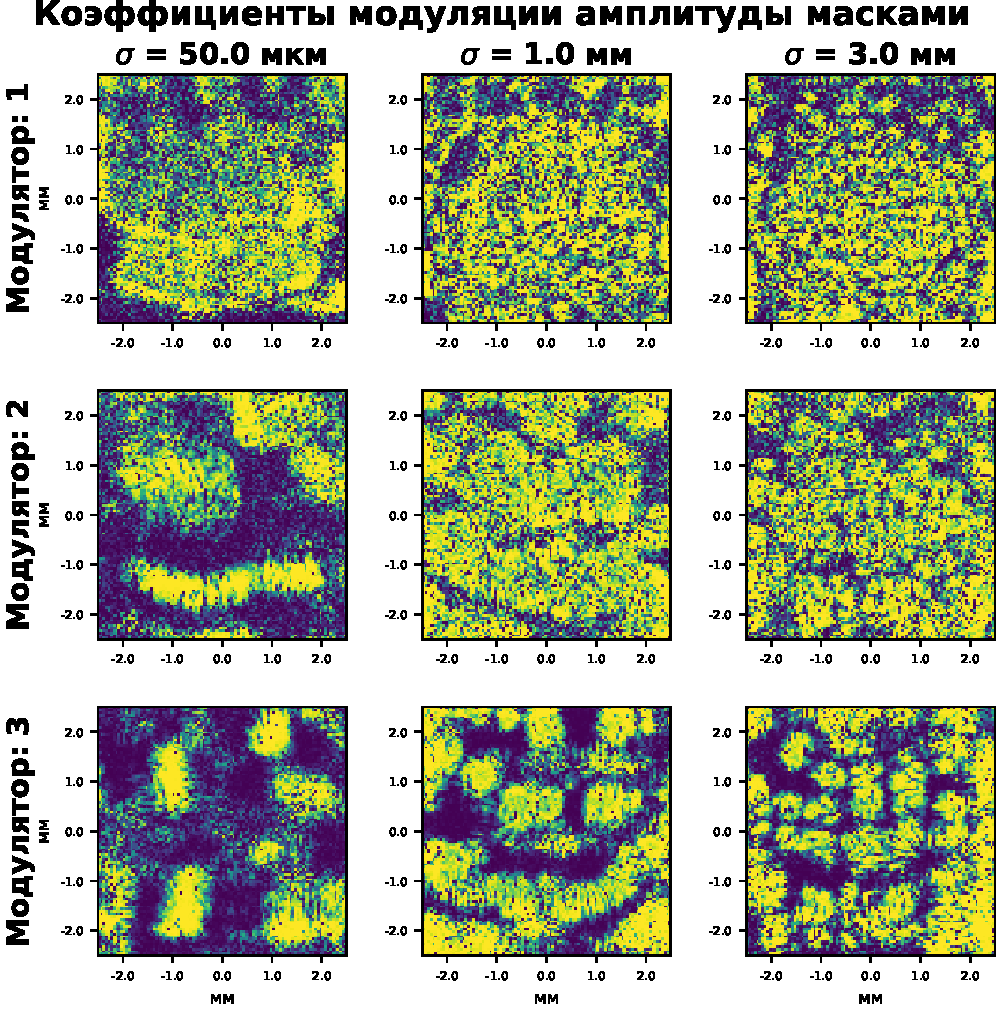
\includegraphics[width=1.0\linewidth]{figures/ModelAmplitude.pdf}}
	\caption{Модуляция амплитуды на неоднородностях масок моделей.}
	\label{ris:ModelAmplitude}
\end{figure}
Фазовые и амплитудные модуляции на этих рисунках далеки от случайного распределения. Это говорит о том, что обучение оптических слоёв реально происходило, что важно потому, что электронная нейронная сеть могла бы обучиться классифицировать зашумленное изображение. Визуально, вид этих рисунков не зависит от степени когерентности, а, скорее всего, определится номером модулирующей маски.
Примеры работы оптоэлектронных нейронных сетей изображены на рисунках \ref{ris:ModelWork1}, \ref{ris:ModelWork2}, \ref{ris:ModelWork3}.
\begin{figure}[h]
	\centering{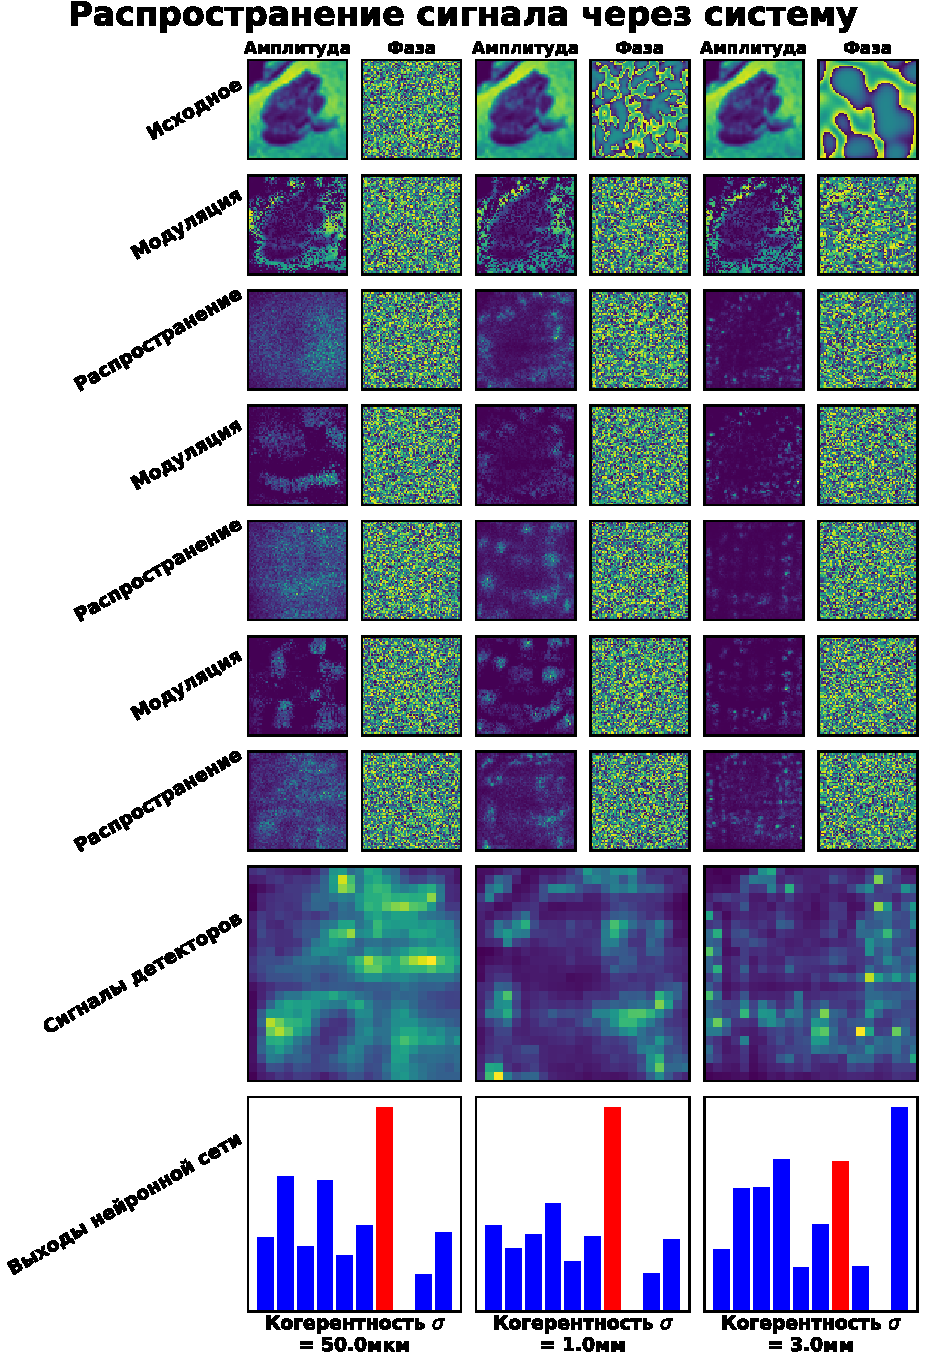
\includegraphics[width=1.0\linewidth]{figures/ModelWork1.pdf}}
	\caption{Прохождение оптического сигнала через оптическую часть гибридной модели, сигналы детекторов и выход электронной нейронной сети.}
	\label{ris:ModelWork1}
\end{figure}
\begin{figure}[h]
	\centering{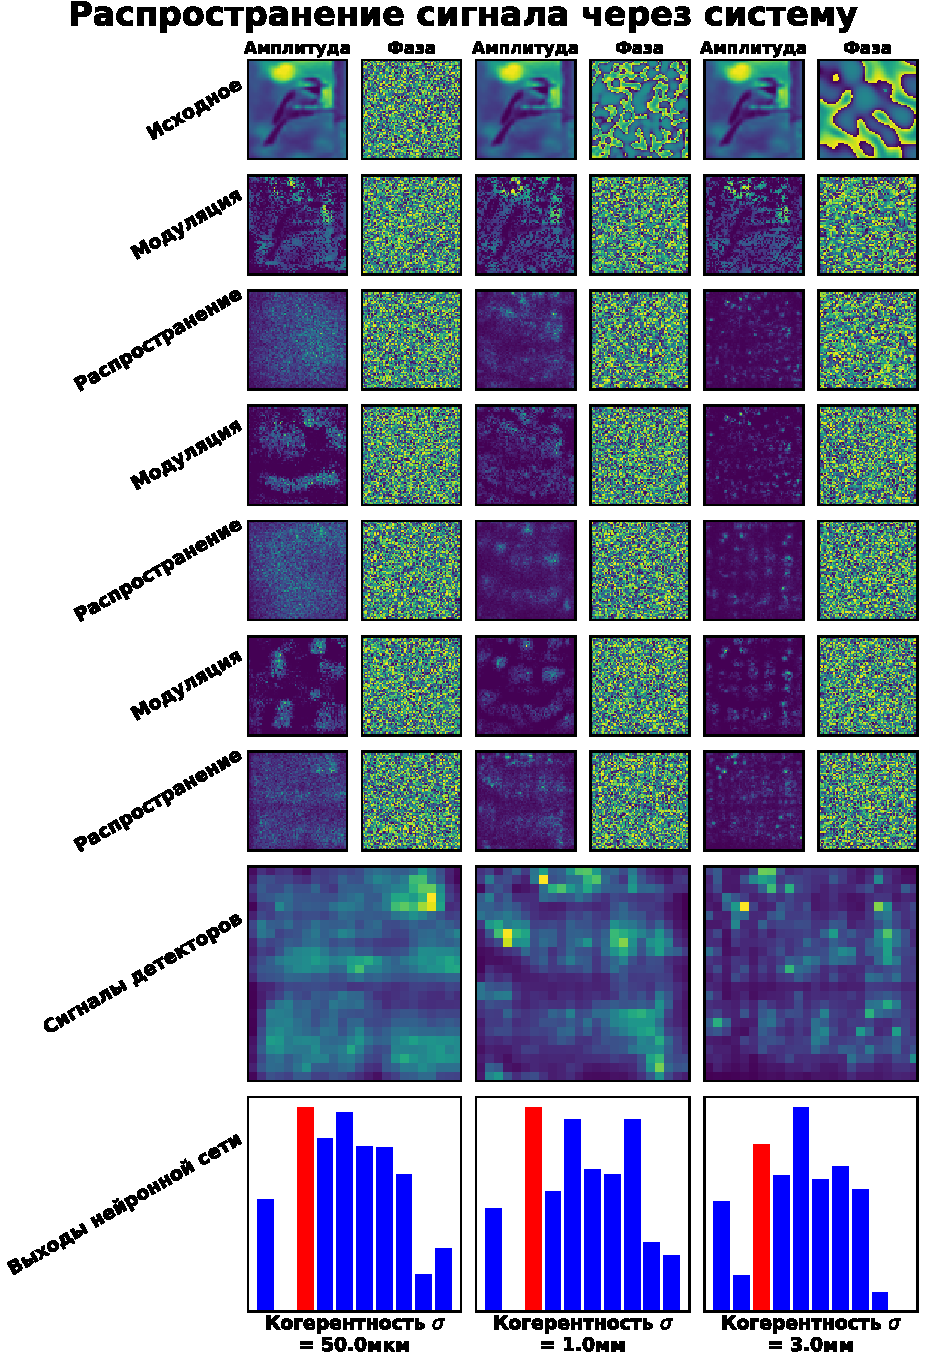
\includegraphics[width=1.0\linewidth]{figures/ModelWork2.pdf}}
	\caption{Прохождение оптического сигнала через оптическую часть гибридной модели, сигналы детекторов и выход электронной нейронной сети.}
	\label{ris:ModelWork2}
\end{figure}
\begin{figure}[h]
	\centering{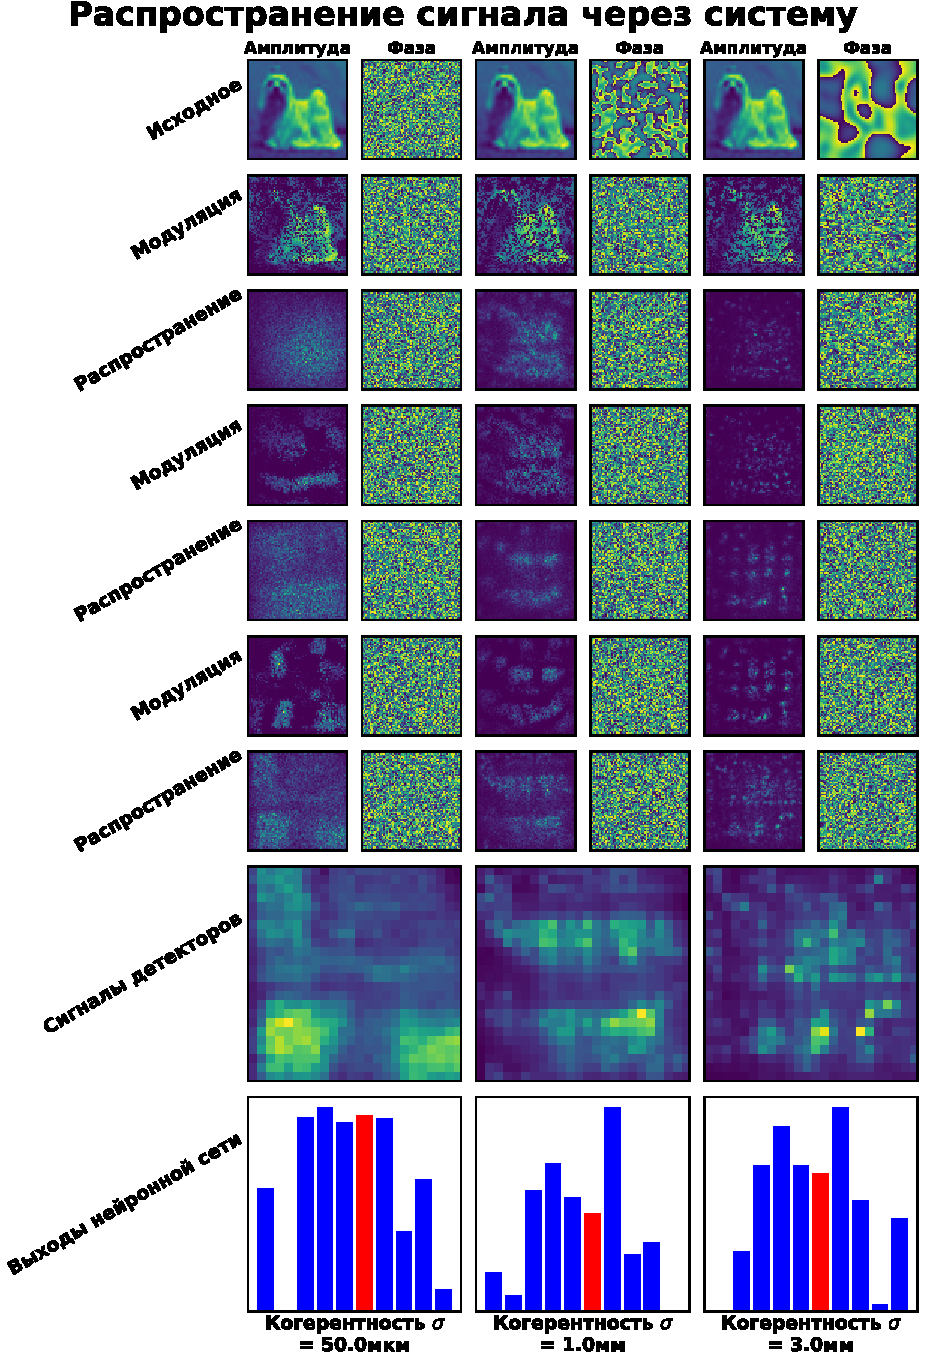
\includegraphics[width=1.0\linewidth]{figures/ModelWork3.pdf}}
	\caption{Прохождение оптического сигнала через оптическую часть гибридной модели, сигналы детекторов и выход электронной нейронной сети.}
	\label{ris:ModelWork3}
\end{figure}
Эти рисунки подтверждают то, что оптическая система не просто пытается сфокусировать изображение на матрицу детекторов, а выполняет некоторые преобразования.